In order to probe the standard model or search for hints of new physics beyond the SM, experiments in particle physics often make use of powerful particle accelerators. In these machines, particles are collided to examine the constituents of matter and interactions between them. The analyses presented in this thesis are performed in the context of the CMS experiment located at the Large Hadron Collider at CERN near Geneva, which is the most powerful accelerator to date. \\ 
The first section of this chapter provides an introduction to the LHC, which is followed by an overview of the detector system of the CMS experiment. Afterwards, the different periods of collision data taking at the LHC are discussed. This chapter concludes with an introduction to the generation of simulated events which are needed for the analysis of real data events.  
\section{The Large Hadron Collider}
\label{sec:lhc}
The LHC~\cite{Bruning:782076, 1748-0221-3-08-S08001} is a ring accelerator designed to provide particle collisions of hadrons. It is built in the tunnel of the former LEP~\cite{LEPdesign} collider 45--170\,m below the surface and has a circumference of 26.7\,km. The LHC is a particle-particle collider and composed of two rings with counter-rotating beams. It can be operated in different modes with either proton or heavy ion (\eg lead) beams.~\footnote{All studies presented in this thesis are based on proton-proton collisions. Thus, the operation with heavy ions is not discussed.} \\
In each beam, protons are grouped together in bunches and accelerated in two evacuated beam pipes using superconducting radio-frequency cavities. With a nominal bunch spacing of 25\,ns, the collision frequency is 40\,MHz. Each of the 2808 individual bunches per beam contains $1.15 \times 10^{11}$ protons, at design conditions. In order to bend the beams around the LHC ring, superconducting dipole magnets are used at a temperature of 1.9\,K. They provide a magnetic field of up to 8.33\,T while additional quadrupole and sextupole magnets are utilized to squeeze and focus the beams.\\  
Before the protons are injected into the LHC, they are pre-accelerated in various smaller accelerators, which are: Linac2, the Proton Synchrotron Booster (PSB), the Proton Synchrotron (PS) and the Super Proton Synchrotron (SPS). With this injector chain, a beam energy of 450\gev is achieved. An overview of the accelerator complex at CERN is given in Fig.~\ref{fig:AccComplex}. 
\begin{figure}[!tp]
  \centering 
  \begin{tabular}{c}
    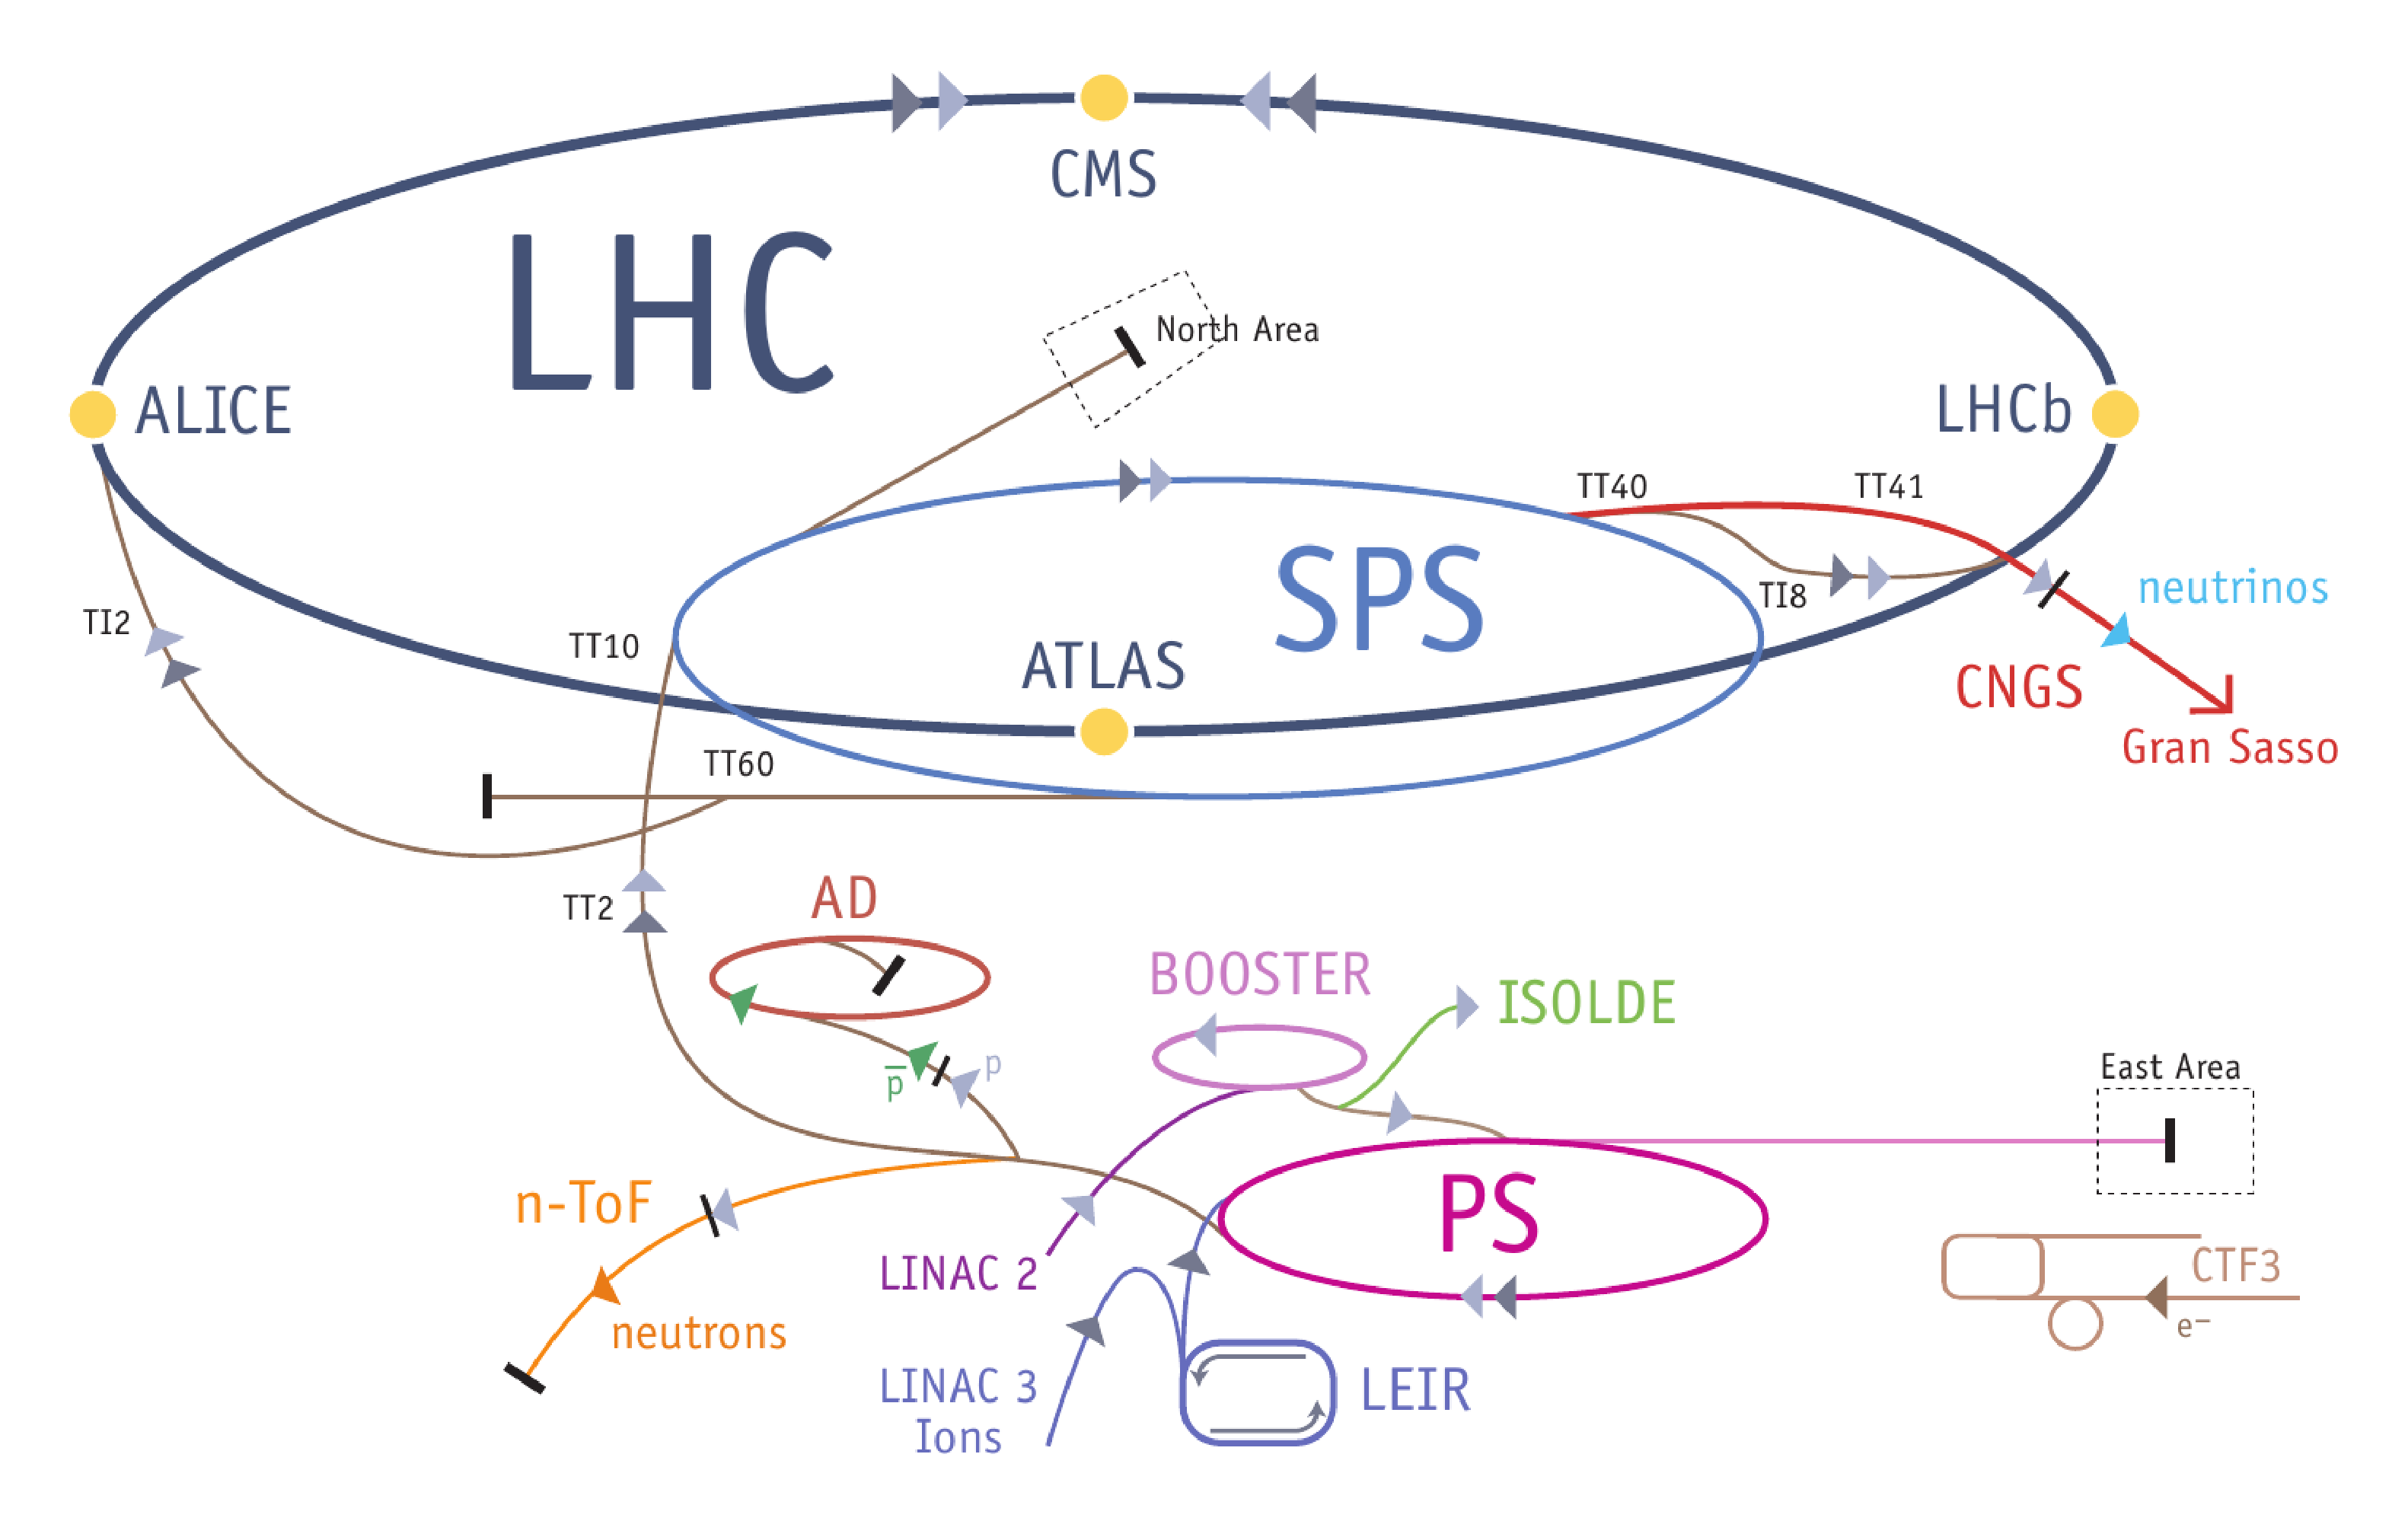
\includegraphics[width=0.9\textwidth]{figures/lhc.pdf}
  \end{tabular}
  \caption{Illustration of the CERN accelerator complex including the injector chain of the LHC ring~\cite{CERNaccelerators}.}
  \label{fig:AccComplex}
\end{figure}
\\
The main goal of the LHC is to provide proton-proton (\pp) collisions to the experiments with centre of mass energies up to 14\tev in order to explore physics processes at novel energy regimes. For a certain process, the expected number of events $N$ is given by the product of the cross section $\sigma$ and the integral $L = \int \mathcal{L}  \, dt$ of the instantaneous luminosity $\cal L$ over time, such that
\begin{equation}
  N = \sigma \cdot L . 
  \label{eq:lumi}
\end{equation}
The luminosity is a machine parameter and can be expressed for beams with Gaussian-shaped profiles as  
\begin{equation}
  \mathcal{L} = \frac{f n_{1} n_{2}}{4 \pi \sigma_{x} \sigma_{y}} \cdot F
  \label{eq:lumi}
\end{equation}
with the collision frequency $f$, the number of particles $n_1$ and $n_2$ contained in the two colliding bunches and the transverse beam sizes $\sigma_{x}$ ($\sigma_{y}$) in the horizontal (vertical) direction. In order to take the inclination of the two beams into account, the geometrical correction factor $F$ is introduced. With design conditions, the nominal peak luminosity of the LHC is $10^{34} \, \mathrm{cm}^{-2} \, \mathrm{s}^{-1}$. Since the total inelastic proton-proton cross-section at a centre of mass energy of 14\tev is around 100\,mb, as indicated in Fig.~\ref{fig:CrossSections}, the expected event rate is approximately $10^9$ events per second. \\
\begin{figure}[!tp]
  \centering
  \begin{tabular}{c}
    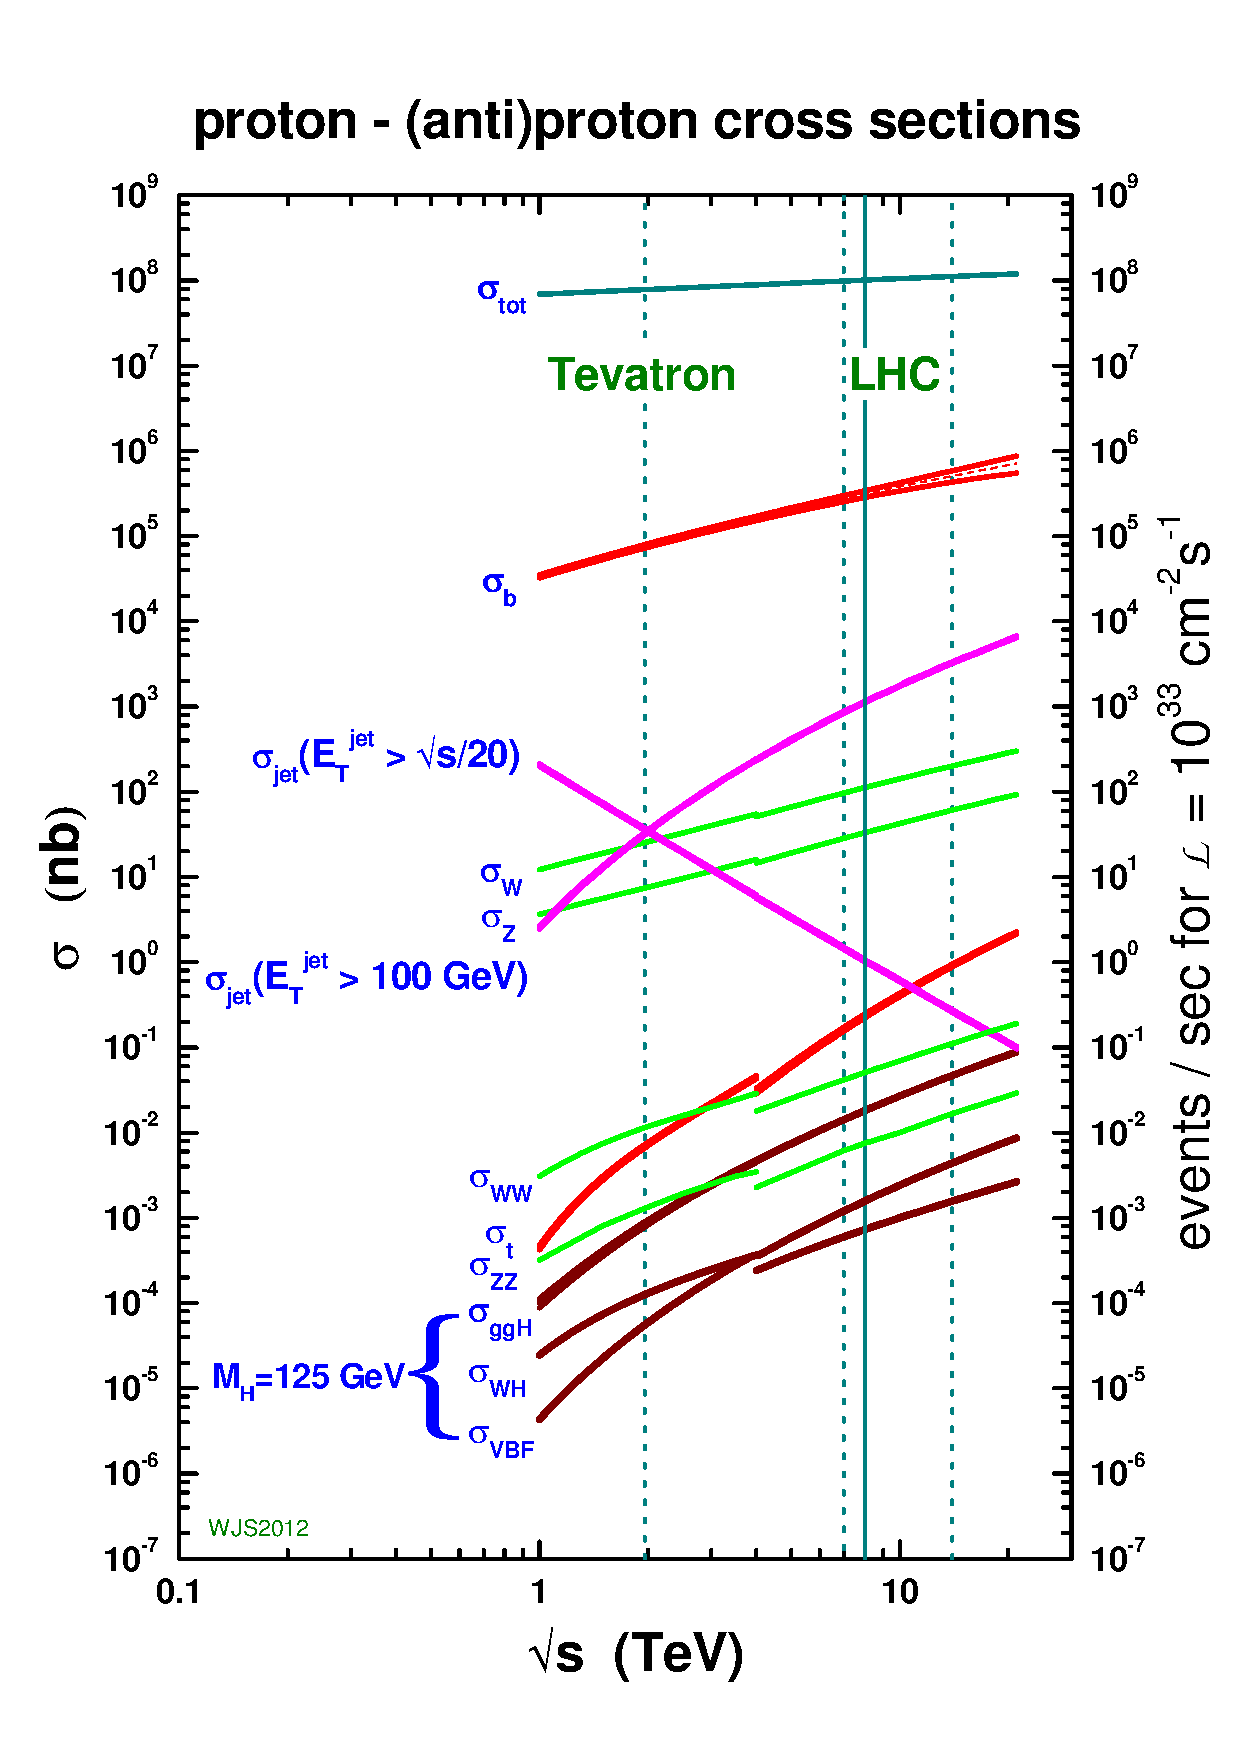
\includegraphics[width=0.60\textwidth]{figures/crosssections2012_v5-1.pdf}
  \end{tabular}
  \caption{Summary of cross sections for various standard model processes in proton-antiproton ($\sqrt{s} < 4$\tev) and proton-proton ($\sqrt{s} > 4$\tev) collisions as a function of the centre of mass energy. The right axis displays the correponding event rate at a luminosity of $\mathrm{10^{33}\,cm^{-2} s^{-1}}$~\cite{bib:stirling:pcom}.}
  \label{fig:CrossSections}
\end{figure}
\\
The four main experiments are located at four of eight locations along the LHC ring where the beams cross and can be brought to collision. The two high luminosity experiments ATLAS~\cite{det::ATLAS} and CMS~\cite{Chatrchyan:2008zzk, bib:cmsptdr1} are designed for multiple purposes like precision measurements of SM quantities, search for the standard model Higgs Boson and searches for signals indicating new physics. The LHCb detector~\cite{det::LHCb}, however, is a specialised experiment and focuses on the measurement of CP violation in the interactions of hadrons containing b quarks. The only experiment especially designed for the analysis of heavy ion collisions is the ALICE~\cite{det::ALICE} detector with the main emphasis on the physics of strongly interacting matter at extreme energy densities, like quark-gluon plasma.

\section{The CMS Experiment}
\label{sec:cms}
The CMS detector is one of the two general-purpose experiments at the LHC. In addition to tests of the SM at the TeV scale, studies of the nature of elektroweak symmetry breaking and searches for so far unknown effects are the primary targets of these experiments. These ambitious goals can only be achieved by fully exploiting the provided collision energy and luminosity with a suitable detector concept.\\
The CMS detector with its typical cylindrical design of different sub-detector components around the beam line is designed to meet these requirements. A sketch of the CMS detector and the different sub-detectors is shown in Fig.~\ref{fig:CMS}.
\begin{figure}[!tp]
  \centering
  \begin{tabular}{c}
    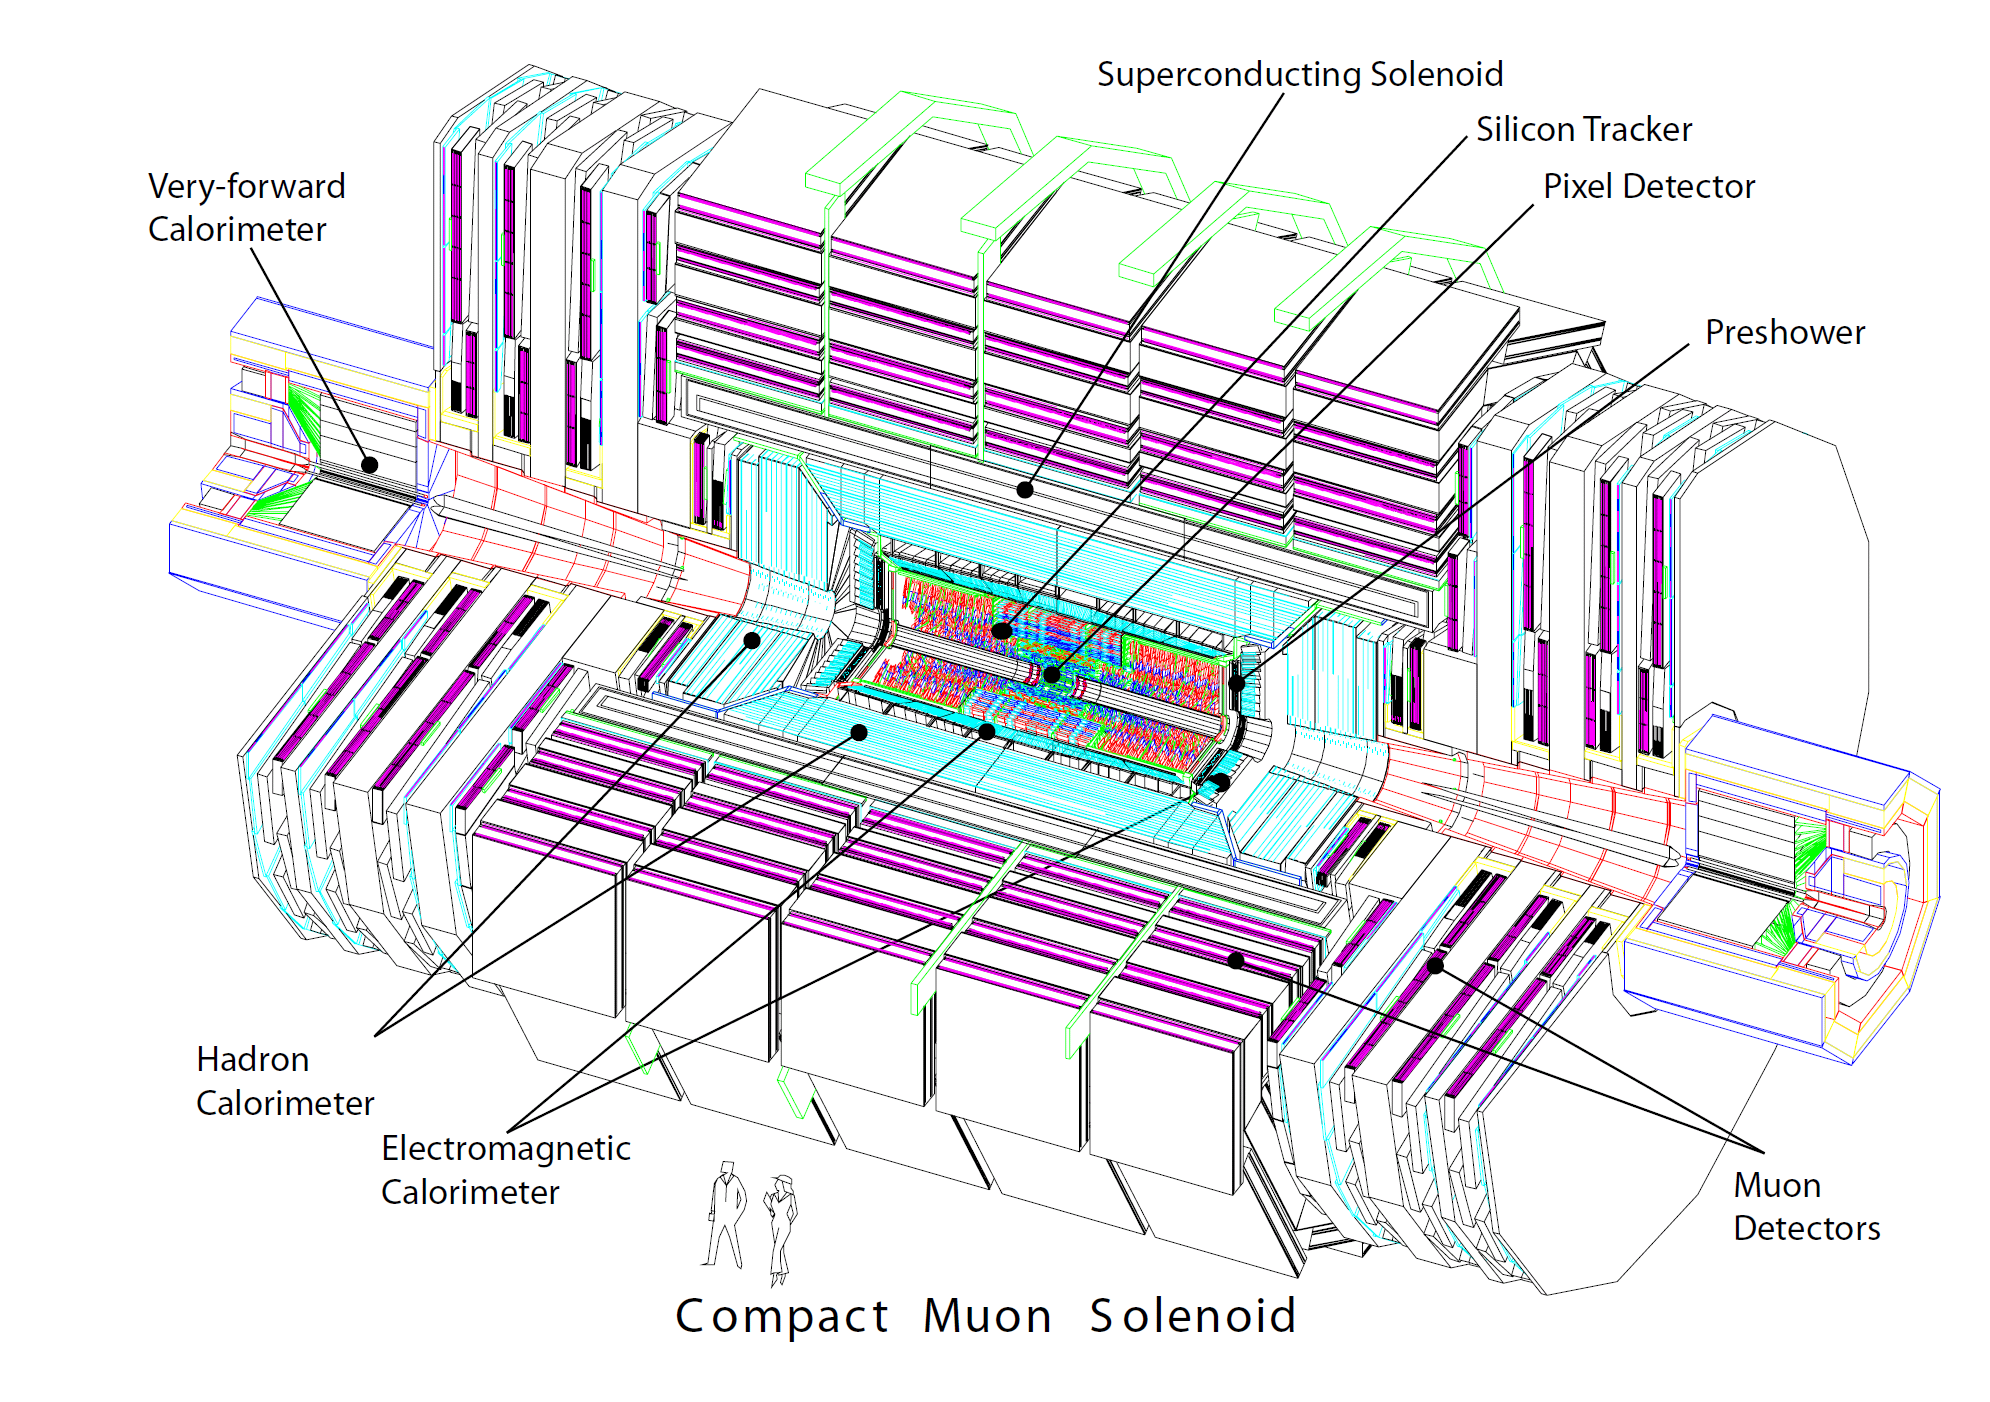
\includegraphics[width=0.99\textwidth]{figures/Figures_Experimental_Apparatus_CMS_perspective.png}
  \end{tabular}
  \caption{A perspective view of the CMS detector~\cite{Chatrchyan:2008zzk}.}
  \label{fig:CMS}
\end{figure}
Such as other high-energy particle experiments, the CMS detector makes use of tracking detectors and calorimeters to measure momenta of particles, energy depositions and flight directions in order to identify the objects emerging from the particle collisions. \\
A typical characteristic of calorimeters is given by the ratio $e/h$. This quantifies the relation between the detection efficiencies of electromagnetic ($e$) and hadronic ($h$) energy deposits in a particle shower. Often it is determined from the ratio of the calorimeter response to pions and electrons $\pi/e$ of the same energy
\begin{equation}
\frac{\pi}{e} = \frac{f_\mathrm{em}\, e + (1 - f_\mathrm{em}) h}{e} = \frac{1+(e/h - 1) f_\mathrm{em}}{e/h}
\end{equation}
with the \textit{electromagnetic fraction} $f_\mathrm{em}$, \ie the fraction of the hadronic shower transferred into an electromagnetic component via the decay of neutral pions into two photons initiating an electromagnetic shower. Since $f_\mathrm{em}$ depends on the energy, the same holds true for $\pi/e$ and the calorimeter response is said to be \textit{non-linear}. \\
Furthermore, the calorimeter performance can be characterized by the relative calorimeter energy-resolution
\begin{equation}
\frac{\sigma(E)}{E}= \frac{N}{E} \oplus \frac{S}{\sqrt{E}} \oplus C 
\end{equation}
which improves with increasing energy $E$ of the measured particle. At low momenta, the resolution is mainly dominated by electronic noise, described by the \textit{noise term} $N$. For increasing energies, the resolution is driven by fluctuations of the shower development described by the \textit{stochastic term} $S$ and at high energies, the resolution is eventually limited by calorimeter miscalibration and non-uniformities described by the \textit{constant term} $C$.\\ 
\\ 
The following sections comprise a description of the CMS detector which exhibits a total weight of 12\,500\,t and has a length of 21.6\,m and a diameter of 14.6\,m. A detailed discussion of the detector design can be found in~\cite{Chatrchyan:2008zzk, bib:cmsptdr1}. After the introduction of the CMS coordinate conventions in Sec.~\ref{subsec:cms_coordinates}, the superconducting magnet is discussed (Sec.~\ref{subsec:cms_magnet}). Afterwards, the tracking system (Sec.~\ref{subsec:cms_tracker}), the calorimeters (Sec.~\ref{subsec:cms_ecal} and~\ref{subsec:cms_hcal}) and the muon system (Sec.~\ref{subsec:cms_muon}) are described moving from the inside of the detector outwards. The detector description ends with a short review of the trigger system in Sec.~\ref{subsec:cms_trigger}.  

\subsection{Coordinate Conventions and Kinematic Variables}
\label{subsec:cms_coordinates}
In order to describe the particle collisions, the CMS experiment makes use of a right-handed coordinate system with its origin at the centre of the detector at the nominal interaction point. While the $z$-axis is defined along the direction of the anti-clockwise beam, the $x$-axis points to the center of the LHC ring and the $y$-axis vertically upwards. In this $xy$-plane the azimuthal angle $\phi$ is measured where $\phi = 0$ coincides with the x-axis. The polar angle $\theta$ is defined with respect to the positive $z$-axis. A quantity closely related to the polar angle is the pseudorapidity $\eta$ defined as
\begin{equation}
\eta = \mathrm{-ln} \left[\mathrm{tan} \left(\frac{\theta}{2} \right)\right]
\end{equation}
which is widely used in experimental particle physics. A pseudorapidity $\eta = 0$ corresponds to the direction perpendicular to the beam while $|\eta| \rightarrow \infty$ points along the beams. Based on the pseudorapidity, the distance between two objects $\Delta R$, which is invariant under Lorentz boosts in $z$-direction, can be written as
\begin{equation}
\Delta R = \sqrt{(\Delta \eta)^2 + (\Delta \phi)^2} \, .
\end{equation}
At the LHC, the hard interaction, \ie the actual momentum transfer, is not taking place between the protons as a whole, but rather between the partons. Since the partons carry an unknown fraction of the proton momenta, the initial conditions of the primary collisions are unknown as well. Thus, conservation of the total momentum can not be utilized directly to describe the momentum balance in the final state. However, it is known that the initial particles have no significant momentum orthogonal to the beam axis which is referred to as \textit{transverse momentum}. Consequently, the transverse momentum of a particle is defined as 
\begin{equation}
\pt = \sqrt{p_x^2 + p_y^2} 
\end{equation}
with the components $p_x$ and $p_y$ of the momentum vector in the $x$ and $y$ direction. Momentum conservation in the transverse plane is then used to constrain the final state. Hence, the momentum imbalance in the transverse plane (\metvec) is determined as the negative vector sum of the momenta of all $N$ particles in the event
\begin{equation}
\metvec = - \sum_{i=1}^{N} \vec{p}_\mathrm{T,i} \; .
\end{equation}
The absolute value of the vector momentum imbalance \met is typically termed \textit{missing transverse momentum} or \textit{missing transverse energy} and serves as estimate for the sum of the transverse momenta of all undetected particles.

\subsection{Superconducting Magnet}
\label{subsec:cms_magnet}
The CMS experiment makes use of a large superconducting solenoid magnet which is a crucial component of the detector design. This magnet provides a uniform magnetic field in $z$ direction of up to 4\,T and allows to precisely determine the momenta and the sign of the charge of charged particles from the curvature in the $(x, y)$-plane of the bended tracks, since it surrounds the tracking and calorimeter systems.\\
With a length of 12.5\,m and a diameter of the free bore of 6.3\,m, the total cold mass reaches 220\,t. The magnet is made up of a niobium-titanium coil which is winded in four layers. This configuration allows a storage of 2.6\,GJ energy at full current. \\
In addition, the muon system located outside of the solenoid is interleaved with a 10\,000\,t heavy-weight iron yoke which is used for the return of the magnetic flux and closes the magnetic field lines. By instrumenting it, this offers the opportunity to measure muon momenta precisely.  

\subsection{Inner Tracking System}
\label{subsec:cms_tracker}
The tracking system of the CMS experiment is the innermost part of the detector and installed directly around the interaction point completely contained in the bore of the magnet system. Its purpose is to precisely measure the trajectories of charged particles arising from the collisions. Furthermore, it is used to identify primary as well as secondary vertices. Due to the location close to the interaction point, the tracking system has to cope with a high particle flux. Hence, high requirements on response time and granularity are set to properly identify particle tracks. \\
In order to fulfill these tasks, the CMS experiment makes use of a tracker design based on silicon detectors. The innermost part is made of silicon pixel detectors. These are surrounded by silicon strip modules. In total, they add up to an active area of 200\,$\mathrm{m}^2$ with a length of 5.8\,m and a diameter of 2.5\,m, covering the detector region up to $|\eta| = 2.5$. A schematic overview of the whole tracking system is shown in Fig.~\ref{fig:CMS_tracker}. 
\begin{figure}[!tp]
  \centering
  \begin{tabular}{c}
    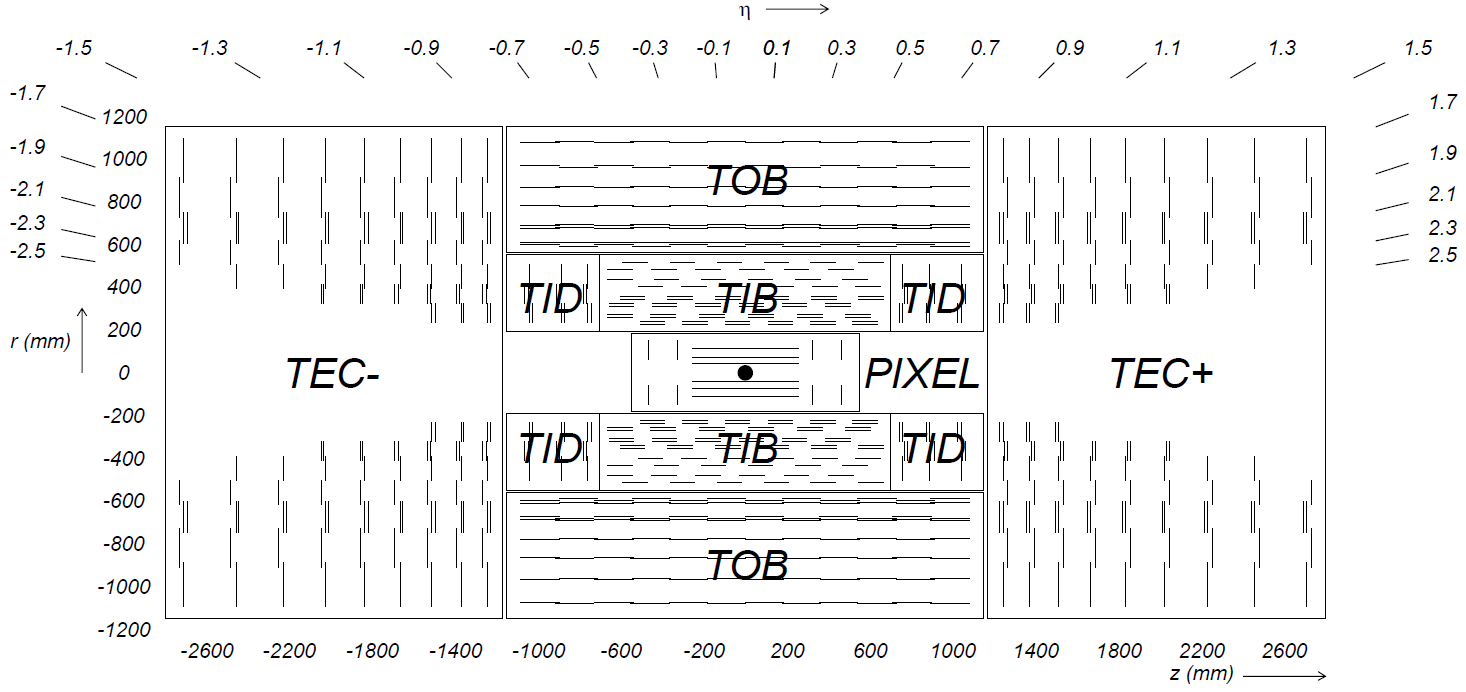
\includegraphics[width=0.95\textwidth]{figures/Figures_Experimental_Apparatus_Tracker.png}
  \end{tabular}
  \caption{Sketch of the CMS tracking system in a $rz$-view. Each tracker module is represented by one line~\cite{Chatrchyan:2008zzk}.}
  \label{fig:CMS_tracker}
\end{figure} 
\begin{description}
 \item \textbf{Pixel Detector:} The pixel detector consists of three barrel layers extending radially from 4.4\,cm to 10.2\,cm and two endcap disks on each side. In total, there are 1440 pixel modules installed. The size of one pixel cell is 100 x 150 \textmu m$^2$ providing similar track resolution quality in $r$--$\phi$ and $z$ direction. This configuration provides for almost the whole range up to $|\eta| = 2.5$ three precise hits which is especially important for the reconstruction of secondary vertices.
 \item \textbf{Silicon Strip Tracker:} The silicon strip detector which extends to a radius of 1.1\,m surrounds the pixel tracker. The more than 15\,000 individual strip detector modules are arranged in an inner and an outer detector part. The inner part of the strip tracker is build by the four \textit{Tracker Inner Barrel} (TIB) layers which are accompanied by the three \textit{Tracker Inner Disks} (TID) at the end sides. This inner part provides up to four track measurements in the $r$--$\phi$ plane. The TIB/TID system lies within the \textit{Tracker Outer Barrel} (TOB) consisting of another six barrel layers while it is complemented by the \textit{Tracker End Caps} (TEC) which add another nine disks at each side of the tracking system. This layout provides at least around nine hits within the silicon strip system. 
\end{description}
The tracking system with the design described above provides a precise impact parameter resolution and high tracking efficiency~\cite{bib:cmstdr:tracker}. The impact parameter resolution is of the order of $\lesssim$ 35\,\textmu m in the plane perpendicular to the beam (for particles with \pt$> 10$\gev) and reaches 75\,\textmu m in the longitudinal direction. Furthermore, the track reconstruction efficiency of high energetic electrons is above 90\%, that of charged hadrons up to 95\% (for \pt$> 10$\gev) and that for muons even better than 98\% in the whole covered region up to $|\eta| = 2.5$. This is achieved already for muons with very low transverse momenta around 1\,GeV. Altogether, the relative transverse momentum resolution reaches a level of 1--2\% for high momentum tracks ($\approx$ 100\gev) in the barrel for $|\eta| < 1.6$.
 
\subsection{Electromagnetic Calorimeter}
\label{subsec:cms_ecal}
The CMS experiment makes use of a homogeneous electromagnetic calorimeter (ECAL), in order to precisely measure the energy deposits of electrons and photons. It is installed around the inner tracking system covering a range up to $|\eta| = 3.0$ and consists of lead tungstate (PbW$\mathrm{O}_4$) crystals. These have been chosen as they provide a high density, short radiation length\footnote{The radiation length corresponds to the mean distance after which an electron traversing a material has lost all but $1/e$ of its energy.} $X_0$ and a small Moli\`{e}re radius\footnote{The Moli\`{e}re radius corresponds to the radius of a cylinder containing on average 90\% of the energy deposition of an electromagnetic shower.} $R_m$ and hence allow to build a compact calorimeter with a fine granularity. As 80\% of the scintillation light is emitted within 25\,ns, this allows ECAL operation at the bunch crossing rate of the LHC machine. In order to collect the radiated light, photodiodes are glued to the back of each crystal.\\
An overview of the ECAL layout is shown in Fig.~\ref{fig:CMS_ecal}. The individual sub-components are as follows:
\begin{figure}[!tp]
  \centering
  \begin{tabular}{c}
    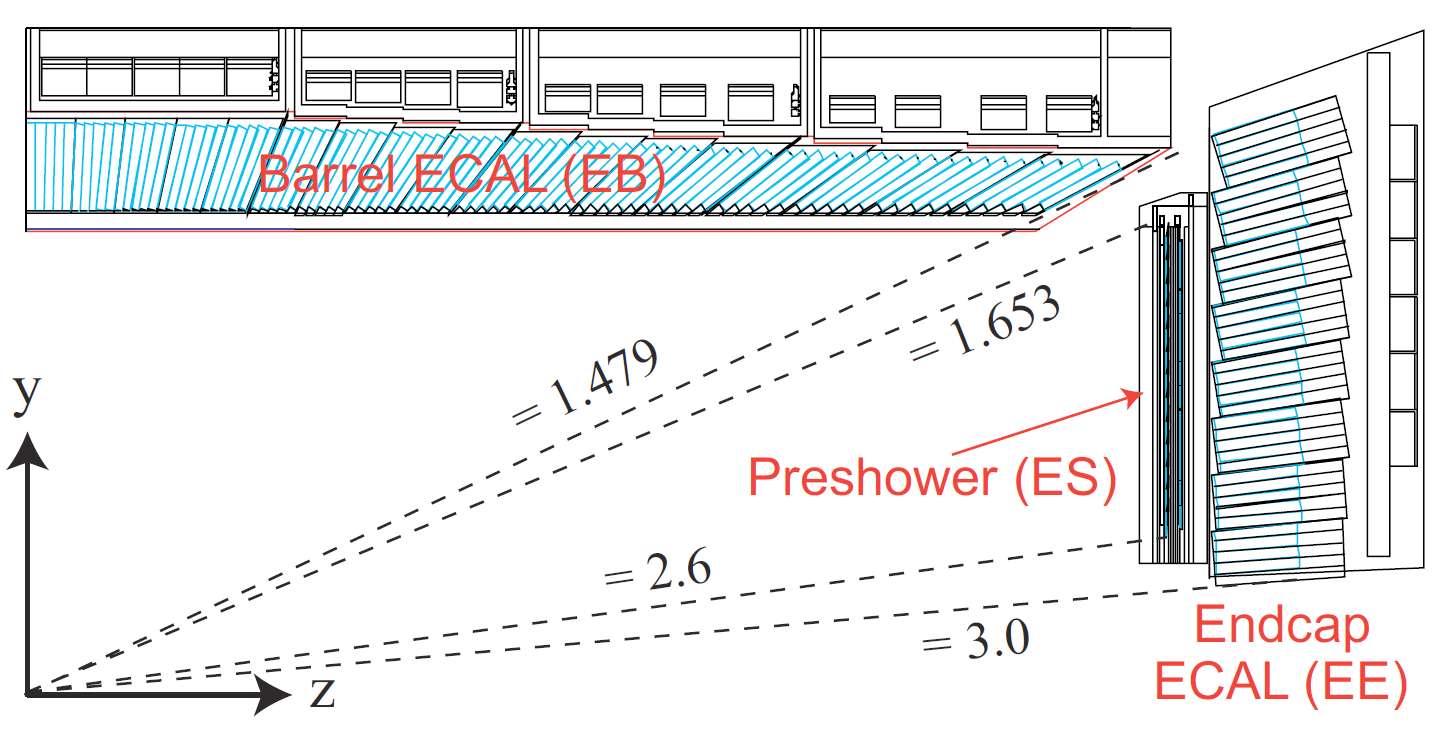
\includegraphics[width=0.95\textwidth]{figures/Figures_Experimental_Apparatus_ECALRapidity.png}
  \end{tabular}
  \caption{View of one quarter section of the CMS electromagnetic calorimeter in a $yz$-view~\cite{bib:cmsptdr1}.}
  \label{fig:CMS_ecal}
\end{figure}
\begin{description}
 \item \textbf{Barrel ECAL (EB):} The barrel detector of the ECAL covers the pseudorapidity region up to $|\eta| = 1.479$. Within a radius of about 1.3\,m, a total number of 61\,200 crystals are installed. Each of them has a length of 230\,mm corresponding to a radiation length of 25.8~$\mathrm{X_0}$. The crystal cross section in $(\eta, \phi)$ is $(0.0174, 0.0174)$. Avalanche photodiodes are used to detect the emitted scintillation light.
 \item \textbf{Endcap ECAL (EE):} The EB is complemented on each side by an endcap which consists of two D-shaped halfs. The ECAL endcaps extend from $|\eta| = 1.479$ to $|\eta| = 3.0$. In total, they contain another 14\,648 crystals. They have an individual length of 220\,mm, which corresponds to 24.7~$\mathrm{X}_0$. For the collection of scintillation light, vacuum phototriodes are used in the endcaps.
 \item \textbf{Preshower (ES):} In front of the endcap crystals, a preshower detector is placed. It covers the pseudorapidity range of $1.653 < |\eta| <2.6$ and is a two-layer sampling calorimeter with lead as absorber material and silicon strip sensors measuring the deposited energy. The total thickness of the preshower is 20\,cm (3~$\mathrm{X_0}$). With its high granularity, it offers the possibility to identify neutral pions decaying into two collimated photons. These constitute an important background contribution in the search for the Higgs boson in the $H \rightarrow \gamma \gamma$ decay channel.
\end{description}
The performance of the ECAL has already been evaluated based on test-beam results~\cite{Abramov:2000vd, springerlink:10.1140/epjc/s10052-009-0959-5}. The ratio $e/h$ has been found to be 1.6 while the relative resolution of electrons with energy $E$ is determined to be
\begin{equation}
\frac{\sigma(E)}{E}= \frac{0.124}{E/\mathrm{GeV}} \oplus \frac{0.036}{\sqrt{E/\mathrm{GeV}}} \oplus 0.0026 \; .
\end{equation}
Thus, the typical relative energy resolution for electrons with a transverse momentum of 120\gev with this calorimeter configuration is of the order of 0.5\%. \\
In addition to the calibration of the absolute energy scale, especially channel-to-channel effects referred to as \textit{intercalibration} have to be accounted for. This intercalibration is performed based on $\pi^0 \rightarrow \gamma \gamma, W \rightarrow e\nu$ and $Z \rightarrow ee$ events and results in a crystal-intercalibration accuracy of 0.6\% ~\cite{CMS-PAS-EGM-10-003}. Changes in the transparency of the ECAL crystals during operation caused by irradiation are monitored by a dedicated laser system based on the injection of reference laser pulses into the crystals. \\

\subsection{Hadron Calorimeter}
\label{subsec:cms_hcal}
The calorimetry of the CMS experiment is completed by the hadron calorimeter (HCAL). It is designed to provide an accurate energy measurement of hadron jets and indirectly also of invisible particles, \eg neutrinos, by the determination of missing transverse energy. In order to measure the missing transverse energy, it is important that the calorimeter is hermetic, meaning that it provides a large geometric coverage to measure all particles emerging from an interaction. Thus, the HCAL is build such that a pseudorapidity range up to $|\eta| = 5.2$ is enclosed. \\ 
The hadron calorimeter completely surrounds the inner tracking system and the electromagnetic barrel calorimeter while it is mainly contained within the magnet system. Hence, its radial dimensions are limited on the one hand by the outer circumference of the barrel ECAL and on the other hand by the inner border of the magnet coil. Thus, an additional calorimeter component is installed outside the solenoid in the barrel part to reduce effects from shower leakage, \ie compensate for hadronic showers that are not fully contained in the HCAL. \\
An overview of the layout of the CMS hadron calorimeter is shown in Fig.~\ref{fig:CMS_hcal}. It is a typical sampling calorimeter with alternating layers of absorber material and active scintillator layers. The individual sub-components are:
\begin{figure}[!tp]
  \centering
  \begin{tabular}{c}
    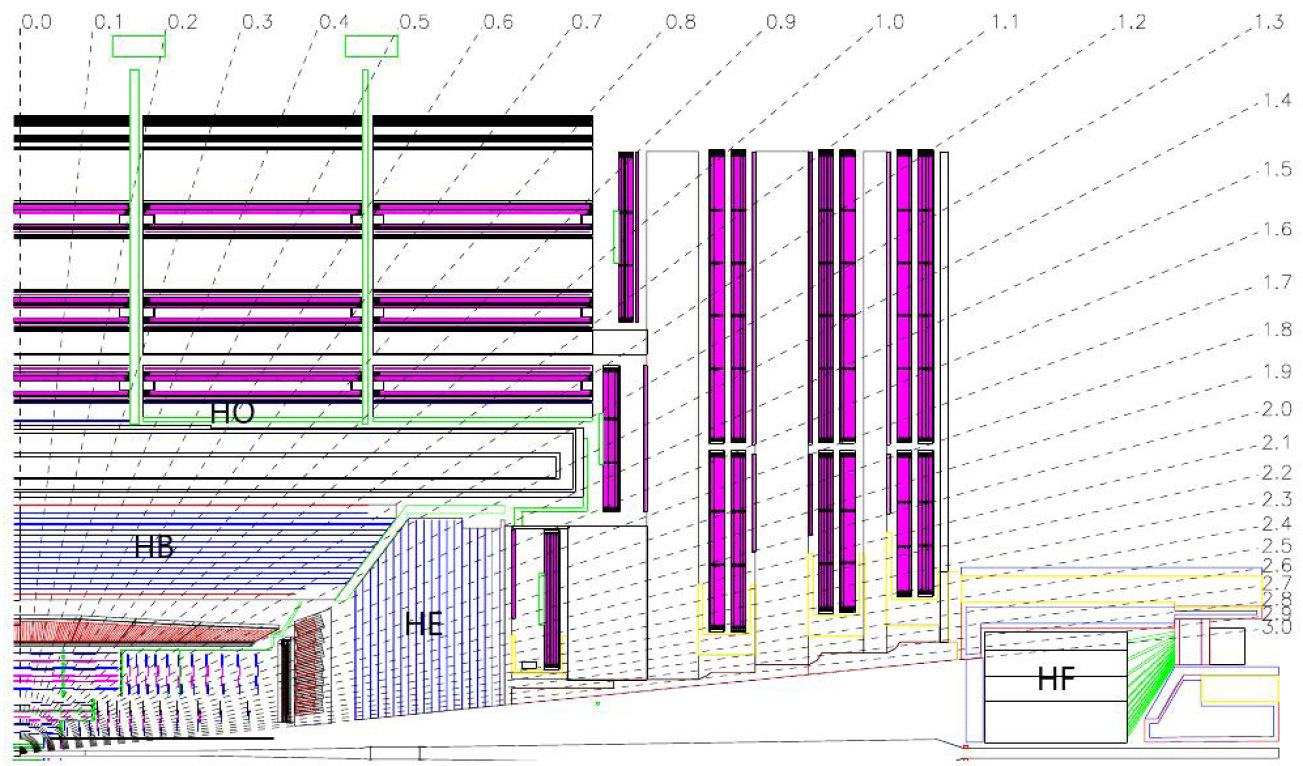
\includegraphics[width=0.95\textwidth]{figures/Figures_Experimental_Apparatus_HCAL.png}
  \end{tabular}
  \caption{Longitudinal view of one quarter of the CMS detector showing the location of the individual HCAL sub-detector parts~\cite{Chatrchyan:2008zzk}.}
  \label{fig:CMS_hcal}
\end{figure}
\begin{description}
 \item \textbf{Hadron barrel (HB):} The barrel part of the CMS hadron calorimeter covers the pseudorapidity range up to $|\eta| = 1.3$ and is composed of two half barrels each containing 36 identical azimuthal wegdes. These wedges hold the absorber plates which are flat brass plates arranged parallel to the axis of the beam. For reasons of stability, the first and last layers are made of stainless steel. The total thickness of the absorber material ranges from 5.82 interaction lengths ($\lambda_I$) at $|\eta| = 0.0$ to 10.6\,$\lambda_I$ at $|\eta| = 1.3$. The 17 active plastic scintillator layers alternate with the absorber plates and have a segmentation in $(\Delta \eta, \Delta \phi)$ of (0.087, 0.087).\\
Each half barrel is divided into 16 $\eta$-regions for which the individual tiles are optically linked together using wavelength shifting fibres and thus form so-called \textit{HCAL towers}. The read-out of each longitudinal tower is carried out using pixelated hybrid photodiodes.
 \item \textbf{Hadron outer (HO):} The calorimeters in the central pseudorapidity region do not provide a sufficient depth in order to fully contain all hadronic showers. Therefore, the HB is complemented by the outer hadron barrel part which is placed outside the solenoid covering $|\eta| \le 1.26$. The HO makes use of the solenoid as additional absorber material and adds another one or even two layers in the most central part of scintillators to the barrel region. Thus, the total depth is extended to 11.8\,$\lambda_I$ at $\eta = 0$.
 \item \textbf{Hadron endcap (HE):} The hadron barrel calorimeter is supplemented by the hadron endcap. It is mounted on the endcap iron yoke and covers the pseudorapidity region of $1.3 \le |\eta| \le 3.0$ using 18 scintillator layers inserted into brass absorber plates. The granularity of the endcap calorimeter is the same as for the barrel up to $|\eta| = 1.6$ and gets coarser for larger pseudorapidities with $(\Delta \eta, \Delta \phi) \approx (0.17, 0.17)$.
 \item \textbf{Hadron forward (HF):} The forward hadron calorimeter extends the pseudorapidity coverage from $|\eta| = 2.9$ (slightly overlapping with the HE) up to $|\eta| = 5.2$. It is located 11.2\,m from the nominal interaction point and has to be radiation hard to cope with the vast particle flux. Thus, the HF is made of steel absorber plates with radiation hard quartz fibres integrated as active material. These fibres are arranged parallel to the beam line and form towers with a size in $(\Delta \eta, \Delta \phi)$ of $\approx$ (0.175, 0.175). The signal is detected as Cerenkov light originating from the quartz fibres.
\end{description}
The HCAL performance has been measured based on test-beam data as well~\cite{Abramov:2000vd, springerlink:10.1140/epjc/s10052-009-0959-5}. From the measurement of the HCAL response to pions and electrons, the ratio $e/h = 1.4$ is extracted and the relative energy resolution of the combined ECAL and HCAL system is determined as
\begin{equation}
\frac{\sigma(E)}{E}= \frac{1.2}{\sqrt{E/\mathrm{GeV}}} \oplus 0.069  
\end{equation}
which corresponds to a relative energy resolution of roughly 14\% for pions with an incident energy of $E = 100$\gev. \\
Similar to the ECAL, also the performance of the HCAL has to be well monitored during operation. Thus, an initial calibration using a radioactive source is combined with test beam data to derive the absolute energy scale. A continous update of this calibrations is performed using isolated energetic particles, \eg from decays of $W$ or $Z$ bosons. 

\subsection{Muon System}
\label{subsec:cms_muon}
The outermost part of the CMS detector, as seen from the interaction point, is made up of the muon system. This component of the detector is assembled in the return yoke of the CMS magnet and consists of a central barrel cylinder complemented by endcap disks in the forward region. This results in a coverage of the pseudorapidity range up to $|\eta| = 2.4$. In the barrel part, four layers of detectors are installed alternating with the iron yoke while the detectors in the endcap are mounted on four discs perpendicular to the beam. In total, about 25\,000\,$\mathrm{m}^2$ detection planes are employed. The layout of the muon system is illustrated in Fig.~\ref{fig:CMS_muon}. \\
Three different types of gaseous detectors are used to achieve a good muon momentum resolution given the different radiation conditions and variations in the homogenity of the magnetic field depending on the pseudorapidity. The different types of tracking chambers are:
\begin{figure}[!tp]
  \centering
  \begin{tabular}{c}
    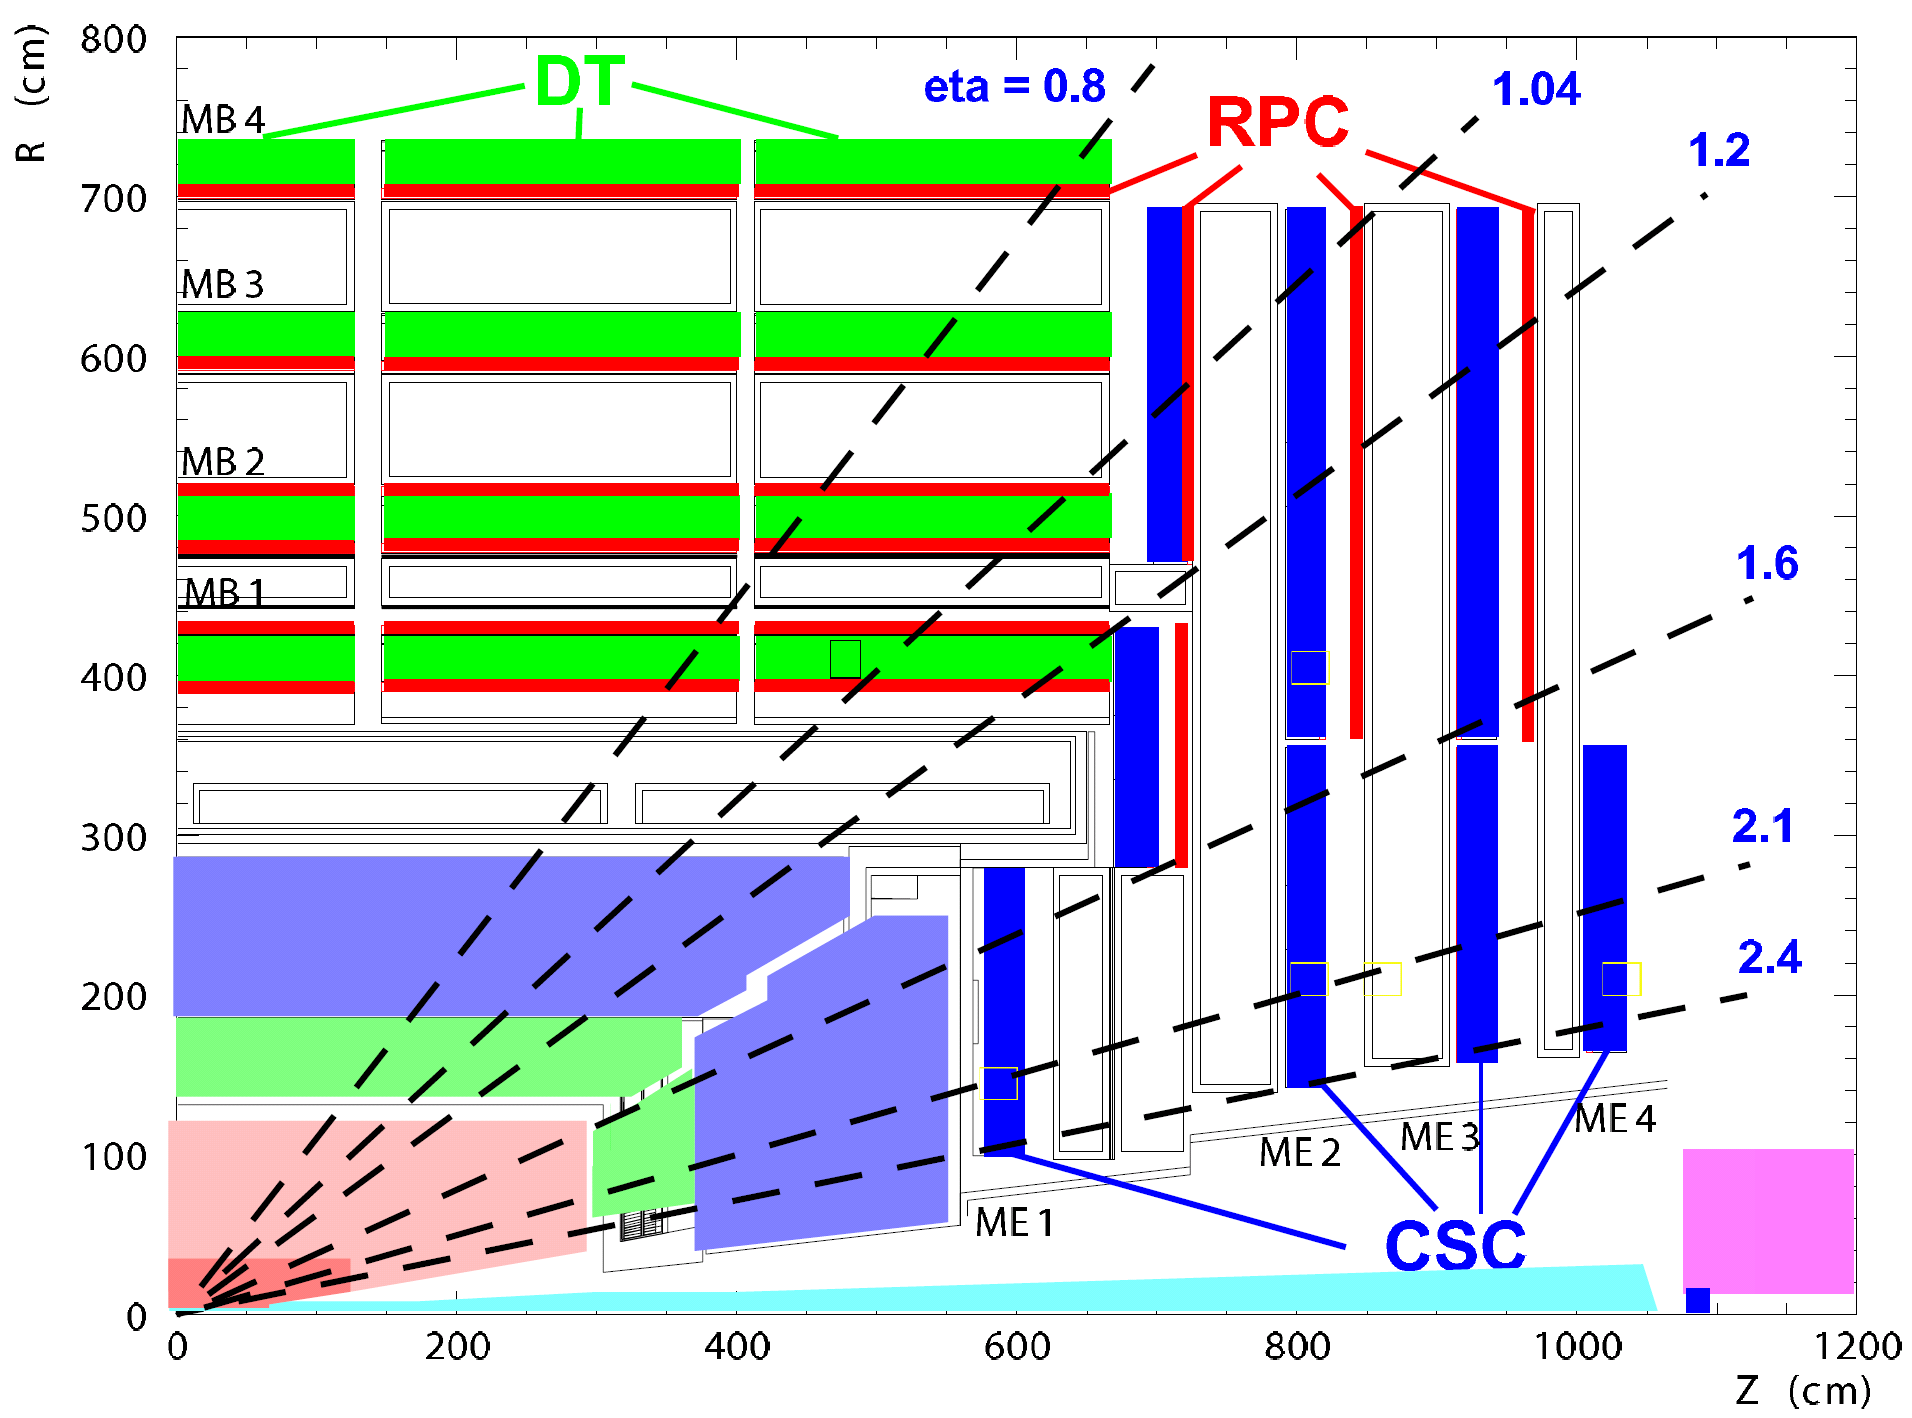
\includegraphics[width=0.95\textwidth]{figures/Figures_Experimental_Apparatus_MuonDetector.png}
  \end{tabular}
  \caption{View of one quarter section of the muon system in the $rz$-plane~\cite{bib:cmsptdr1}.}
  \label{fig:CMS_muon}
\end{figure}

\begin{description}
 \item \textbf{Drift tube (DT) chambers:} In the barrel region for $|\eta| < 1.2$, the background due to neutrons is low and likewise residual effects from the magnetic field. Here, the muon system is equipped with drift tube chambers. In the barrel, the muon coordinates in the $r\phi$-plane are measured in four stations while only the first three layers provide also a measurement of the $z$-direction. The drift length is restricted to a maximum of 21\,mm resulting in a negligible occupancy while keeping the number of channels at an acceptable level. Furthermore, a technology based on tubes is chosen avoiding the issue of possibly broken wires. The resolution in $r\phi$ is designed to reach a precision of 100\,\textmu m.
 \item \textbf{Cathode strip chambers (CSC):} The endcap regions are equipped with cathode strip chambers and cover the pseudorapidity range $0.9 < |\eta| < 2.4$. These provide a fast response time and fine segmentation while they are resistant against radiation. Thus, they are well suited for the forward region where the muon and background rates are largely increased and the magnetic field is high and non-uniform. The CSCs, which are multiwire proportional chambers in which anode wires are interlaced with cathode panels, perform a precise position measurement in the $r\phi$--plane with a spatial resolution of 75--150\,\textmu m. 
 \item \textbf{Resistive plate chambers (RPC):} Resistive plate chambers are used to complement the drift tube and cathode strip chambers in the range $|\eta| < 1.6$. These are gaseous parallel-plate detectors with a spatial resolution coarser than the DTs and CSCs. However, they provide a very fast response and good time resolution at high particle rates. Thus, they are able to very efficiently detect the bunch-crossing a muon track is associated to. 
\end{description}
The global muon reconstruction efficiency is in general about 95--99\% and only drops for some $|\eta|$ regions, \eg in the transition region between the barrel and endcap part around $|\eta|=1.2$. Since muons reaching the muon system are affected by multiple scattering and radiation losses in the material, the resolution for muons with transverse momenta below $\approx$ 200\gev is in general better based on the inner tracking system than for the muon system. However, at higher transverse momenta the track-curvature measurement in the inner tracking system is limited and thus a combination with the measurement in the muon system beneficial due to the longer lever arm. In general, the muon momentum resolution can be improved by combining the information from the inner tracker and the muon system due to an improved fault finding. This combined approach results in a relative muon momentum resolution for muons with high momenta around 1\tev of about 5\%.

\subsection{Trigger System}
\label{subsec:cms_trigger}
The LHC operating at design conditions provides particle collisions with a bunch crossing rate of 40\,MHz. This results in an enormous amount of event data which have to be processed and stored for later analyses. With an approximate event size of 1\,MB, it is technically impossible to record all events. However, as illustrated in Fig.~\ref{fig:CrossSections}, the event rate of interesting events is orders of magnitudes smaller than the total inelastic proton-proton cross section. Thus, already in the trigger system a fast event preselection is performed that allows to reduce the amount of data to a storable size while still retaining the information of interest. Hence, the trigger system makes up the first step in the physics analysis process.\\
In order to achieve the necessary rate reduction, the CMS experiment uses a two-stage trigger system:
\begin{description}
\item \textbf{Level-1 (L1) trigger:} The L1 trigger consists of custom-made fast programmable hardware. It makes use of data received from fast detector components which are the calorimeters and the muon system at reduced granularity. For that purpose, the calorimeter is divided into so-called \textit{trigger towers} which cover an area in $(\eta, \phi)$ of $(0.087, 0.087)$ up to $|\eta| = 1.74$ getting even coarser for higher $|\eta|$. At L1, the trigger decision is based on energy deposits in those trigger towers or certain hit patterns in the muon chambers forming trigger primitive objects which are electrons/photons, muons or jets and global quantities like sums of \et or \met. Events are accepted, if thosee trigger objects pass some predefined criteria like for instance certain \pt thresholds. The L1 trigger latency, \ie the time between the actual bunch crossing and the delivery of a positive L1 trigger decision to the front-end electronics, is 3.2\,\textmu s. During this period, the high resolution data is pipelined in readout buffers for further processing. The L1 trigger reduces the event rate to a maximum of 100\,kHz.
\item \textbf{High-Level trigger (HLT):} Events that are accepted by the L1 trigger stage are transferred to the High-Level trigger for further processing. The HLT is a software system running on several thousand commercial processors. It has access to the full information from all sub-detectors and performs an event reconstruction similar to the later event reconstruction performed for recorded data. Thus, it allows a further rate reduction to the final output rate of a few hundred Hz of events that are finally stored for analyses. Since the HLT is software based, it allows to continously adjust the used algorithms in order to adapt to changing conditions during operation.
\end{description}
In the two trigger stages, various different conditions can be tested in parallel which define the so-called \textit{trigger paths}. For instance, there exist dedicated trigger paths to select events with single electrons or muons above a certain \pt threshold or paths to collect events with a specific amount of missing transverse energy. All of these individual trigger paths form together the \textit{trigger menu} and are operated with a dedicated rate such that the total manageable output rate of a few hundred Hz is not exceeded. Typically, the instantaneous luminosity changes gradually during operation which can result in changing output rates for individual trigger paths. In order to not exceed the allowed total trigger rate, the number of recorded events per trigger path can be adjusted accordingly by requiring that only each $n^\mathrm{th}$ triggered event is kept. The respective value of $n$ is denoted \textit{prescale factor}. 

\section{LHC Operation and Data Taking}
\label{sec:data}
\begin{figure}[!t]
  \centering
  \begin{tabular}{c}
    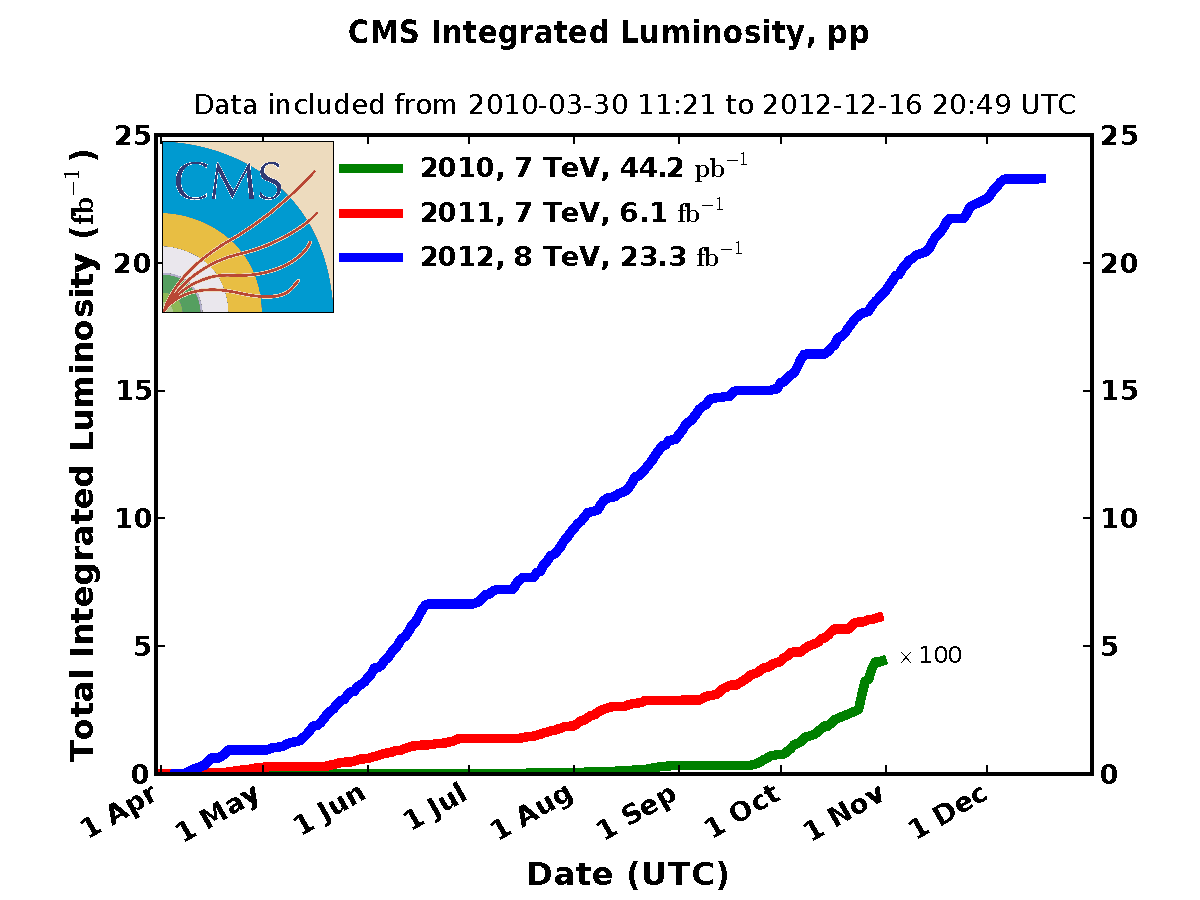
\includegraphics[width=0.95\textwidth]{figures/int_lumi_cumulative_pp_2.pdf}
  \end{tabular}
  \caption{Cumulative integrated luminosity versus day delivered to CMS during stable beams for pp collisions. Different data-taking periods are indicated as follows: green for 2010, red for 2011 and blue for 2012~\cite{bib:lhc:lumi12}.}
  \label{fig:lhc_data}
\end{figure}
The first operation of the LHC took place in September 2008. After a major cooling incident only a few days later requiring a longer technical stop, beams were circulated again in November 2009. The first collisions at a center of mass energy of 7\tev finally happened end of March 2010~\cite{bib:lhcmachineoutreach}. In the following running period in 2010, data corresponding to an integrated luminosity of 44.2\pbinv were delivered to the experiments with a maximum peak instantaneous luminosity of $2.05 \times 10^{32} \cm^{-2} \second^{-1}$. These data allowed studies of the detector performance and made first searches for new physics possible. The next data taking period performed during 2011 at the same centre of mass energy even delivered a total amount of 6.1\fbinv \pp collision data reaching a peak instantaneous luminosity of $3.5 \times 10^{33} \cm^{-2} \second^{-1}$. Following another technical shutdown during winter, the centre of mass energy was finally increased to 8\tev for the running period during 2012 and the peak luminosity reached values of up to $7.7 \times 10^{33} \cm^{-2} \second^{-1}$, which is already almost design conditions. In total, 23.3\fbinv of integrated luminosity \pp collisions were produced by the LHC operating at stable beam conditions. The evolution of the integrated luminosity versus days is illustrated in Fig.~\ref{fig:lhc_data} for data-taking periods in 2010, 2011 and 2012. Typically, these periods are referred to as \textit{LHC Run I}. \\
During most of the operation in 2012, the LHC was circulating 1380 bunches per beam with a spacing of 50\,ns. The average bunch intensity, \ie the number of protons per bunch, was varying from $1.6$ to $1.7 \times 10^{11}$ exceeding even the design value~\cite{bib:lhc:lumi12, Lamont:2013cma}. \\
In general, such conditions result in multiple interactions per bunch crossing known as \textit{pileup} (PU). Typically, two sources of pileup are distinguished: \textit{in-time} pileup (IT PU) and \textit{out-of-time} pileup (OOT PU). While IT PU is caused by additional \pp collisions occuring within the same bunch-crossing as the primary hard collision and leads to additional tracks in the tracking system and energy deposits in the calorimeters, OOT PU arises from \pp collisions in previous and following bunch crossings and contributes further energy deposits in the calorimeters to the hard interaction due to the finite signal decay time in the calorimeters. An overview of the pileup profile in collision data taken in 2012 is given in Fig.~\ref{fig:lhc_pileup}. Here, the mean number of interactions per bunch crossing is illustrated with the mean of this distribution located at 21. The maximum number of mean pileup events even reached a value of $\approx 40$. Dedicated techniques in order to mitigate effects from pileup have been developed of which some are discussed in Chap.~\ref{chap:Objects}.
\begin{figure}[!t]
  \centering
  \begin{tabular}{c}
    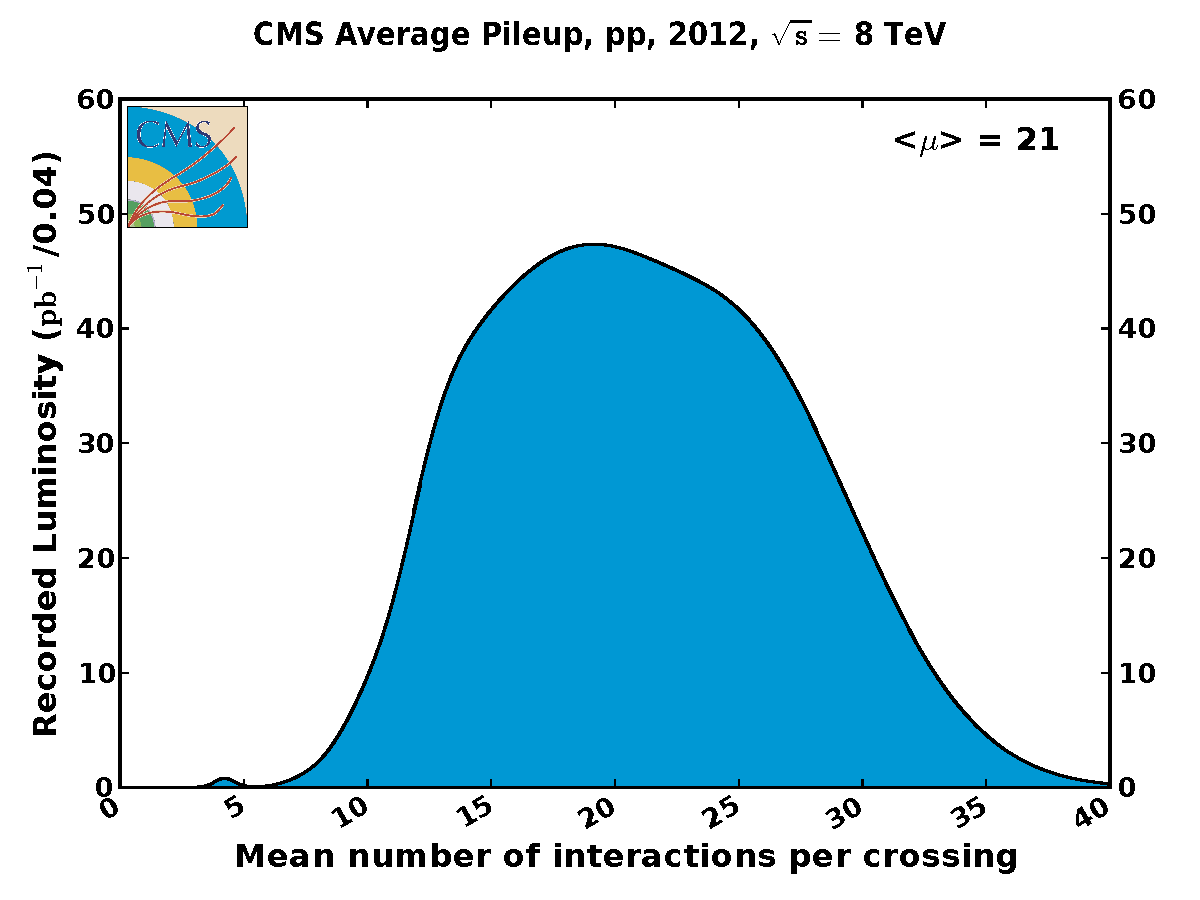
\includegraphics[width=0.95\textwidth]{figures/pileup_pp_2012.pdf} 
  \end{tabular}
  \caption{Mean number of interactions per bunch crossing in \pp collisions at a centre of mass energy of $\sqrt{s} = 8$\tev~\cite{bib:lhc:lumi12}.}
  \label{fig:lhc_pileup}
\end{figure}





